%%
%% Copyright 2007-2020 Elsevier Ltd
%%
%% This file is part of the 'Elsarticle Bundle'.
%% ---------------------------------------------
%%
%% It may be distributed under the conditions of the LaTeX Project Public
%% License, either version 1.2 of this license or (at your option) any
%% later version.  The latest version of this license is in
%%    http://www.latex-project.org/lppl.txt
%% and version 1.2 or later is part of all distributions of LaTeX
%% version 1999/12/01 or later.
%%
%% The list of all files belonging to the 'Elsarticle Bundle' is
%% given in the file `manifest.txt'.
%%

%% Template article for Elsevier's document class `elsarticle'
%% with numbered style bibliographic references
%% SP 2008/03/01
%%
%%
%%
%% $Id: elsarticle-template-num.tex 190 2020-11-23 11:12:32Z rishi $
%%
%%
\documentclass[preprint,12pt, pdftex]{elsarticle}

%% Use the option review to obtain double line spacing
%% \documentclass[authoryear,preprint,review,12pt]{elsarticle}

%% Use the options 1p,twocolumn; 3p; 3p,twocolumn; 5p; or 5p,twocolumn
%% for a journal layout:
%% \documentclass[final,1p,times]{elsarticle}
%% \documentclass[final,1p,times,twocolumn]{elsarticle}
%% \documentclass[final,3p,times]{elsarticle}
%% \documentclass[final,3p,times,twocolumn]{elsarticle}
%% \documentclass[final,5p,times]{elsarticle}
%% \documentclass[final,5p,times,twocolumn]{elsarticle}

%% For including figures, graphicx.sty has been loaded in
%% elsarticle.cls. If you prefer to use the old commands
%% please give \usepackage{epsfig}

%% The amssymb package provides various useful mathematical symbols
\usepackage{amssymb}
\usepackage[utf8]{inputenc}
\usepackage[numbers]{natbib}
\usepackage[spanish,mexico]{babel}
\renewcommand {\spanishtablename}{Cuadro}
\renewcommand{\abstractname}{Resumen}
\usepackage{amsmath}

%% The amsthm package provides extended theorem environments
%% \usepackage{amsthm}

%% The lineno packages adds line numbers. Start line numbering with
%% \begin{linenumbers}, end it with \end{linenumbers}. Or switch it on
%% for the whole article with \linenumbers.
%% \usepackage{lineno}
\usepackage{booktabs}
\usepackage{etoolbox}
\usepackage{fancyvrb}
\usepackage{multirow}
\usepackage{color,soul}
\usepackage[dvipsnames]{xcolor}
\usepackage{graphicx}
\usepackage{subcaption}
\usepackage{listings}
\usepackage{amssymb}
\usepackage{dirtytalk}


\usepackage{verbatim}

% redefine \VerbatimInput
\RecustomVerbatimCommand{\VerbatimInput}{VerbatimInput}%
{fontsize=\footnotesize,
 %
frame=lines,  % top and bottom rule only
framesep=1em, % separation between frame and text
rulecolor=\color{Gray},
 %
label=\fbox{\color{Black}Pruebas.txt},
labelposition=topline,
%
%commandchars=\|\(\), % escape character and argument delimiters for
                  % commands within the verbatim
 %commentchar=*        % comment character
}

\journal{Nuclear Physics B}

\begin{document}

\begin{frontmatter}

\title{Comparación de métodos de solución para la ubicación y recolección de productos en un almacén}

\author{Johanna Bolaños Zuñiga}
\ead{johana.bolanoszn@uanl.edu.mx}
\address{Universidad Autónoma, San Nicolás de los Garza, Nuevo León México}

\renewcommand{\abstractname}{Resumen}
\begin{abstract}
El proceso de preparación de pedidos es uno de los principales problemas en los almacenes, donde una de las actividades con mayor costo operativo es la recolección de pedidos. Esta actividad se logra mediante una política de enrutamiento que determina la secuencia que debe seguir el recolector de pedidos para tomar los artículos de las ubicaciones del almacén. Por lo tanto, las decisiones de asignación del espacio de almacenamiento influyen en la minimización del tiempo de recolección de pedidos y, en consecuencia, en la reducción de los costos de operación del almacén. De acuerdo a lo anterior, se cuenta con un modelo matemático y una metaheurística para determina simultáneamente las decisiones de almacenamiento y rutas de recolección de los productos, considerando restricciones de precedencia con base en el peso del producto y las características del caso de estudio, como tener una única ubicación para cada producto en un almacén con un diseño general. En esta investigación mediante las pruebas de hipótesis sobre la media de la diferencia se resalta que entre los dos métodos propuestos estadísticamente la metaheurística presenta mejores resultados que la solución encontrada hasta el momento por el método exacto para la problemática planteada.
\end{abstract}

\begin{keyword}
Preparación de pedidos \sep Problema del recolector \sep Almacenamiento \sep Prueba de hipótesis \sep Prueba $t$

%% PACS codes here, in the form: \PACS code \sep code

%% MSC codes here, in the form: \MSC code \sep code
%% or \MSC[2008] code \sep code (2000 is the default)

\end{keyword}

\end{frontmatter}

%% \linenumbers Kermack_McKendrick_1927

%% main text
\section{Introducción} \label{introduccion}
Según las necesidades de los clientes, el almacenamiento y el proceso de preparación de pedidos son un componente principal de cualquier cadena de suministro. Desde $1984$ el Consejo de Educación e Investigación de Almacenaje (WERC por sus siglas en inglés de \textit{Warehousing Education and Research Council}) \citep{Goetschalckx1988} identificó que el proceso de preparación de pedidos (conocido como \textit{order picking process}) es la principal área de oportunidad de la industria del almacenamiento. De acuerdo a estudios realizados por \citet{Tompkins2010} y \citet{Henn2013}, es uno de los procesos más críticos a nivel operativo dentro de un almacén, debido a que representa entre el 55\% - 60\% de sus costos, razones por las cuales las empresas se ven obligadas a llevar a cabo esta actividad de la mejor manera posible.

Por otro lado, en la investigación de \citet{Goetschalckx1989}, el nivel de servicio de una empresa se compone de una variedad de factores tales como el promedio y la variación del tiempo de entrega de la demanda, la integridad y la precisión del producto. Por lo tanto, un vínculo crucial entre la preparación de pedidos y el nivel de servicio es que cuanto más rápido se realice la recolección de lo solicitado, más rápido estará disponible para enviarla al cliente. De lo contrario, es posible que se incurra en un atraso de la entrega provocando una mala prestación del servicio e o inconformidad por parte del cliente. No obstante, la empresa podría incurrir en trabajos adicionales para entregar a tiempo, elevando con ellos los costos de esta operación.

La preparación de pedidos implica una serie de actividades que van desde la selección o programación de los pedidos, la recolección de las cantidades de los diferentes artículos desde su ubicación de almacenamiento hasta el despacho de estos, en respuesta a las solicitudes de sus clientes. No obstante, para \citet{Davarzani2016} y \citet{DeKoster2007} los objetivos a alcanzar en la recolección de pedidos son la minimización de las distancias o el tiempo de viaje que los recolectores realizan a través del almacén para cumplir con la demanda, actividades que se llevan a cabo por medio de políticas de enrutamiento, las cuales determinan la secuencia en la que el recolector de pedidos toma los artículos de las ubicaciones del almacén, y especifican tanto el orden en los que estos tienen que ser recogidos, así como el orden en la que se deben de visitar los pasillos. 

Además, de acuerdo a las investigaciones de \citet{Brynzer1996} y \citet{Manzini2012} una correcta ubicación de almacenamiento de los productos facilita la precisión de proceso y la colocación más eficiente de las existencias, consiguiendo ciclos de pedidos más rápidos y con mejor servicio al cliente, lo que convierte al almacenamiento y el enrutamiento en uno de los principales problemas en la práctica. Para este trabajo se cuenta dos métodos de solución (modelo matemático y una metaheurística) para resolver estos problemas de manera conjunta en una empresa donde no existe una ubicación apropiada de los productos, no se recolectan los productos con base a su peso y generan costos extras de personal para evitar incumplimiento de las entregas a los clientes. Se pretende comprobar que existe un ahorro entre la metaheurística y la solución ofrecida hasta el momento por el modelo matemático.

El resto de este trabajo está organizado de la siguiente manera: En la sección \ref{antecedentes} se presenta una revisión de literatura que aborda los temas recolección de pedidos, almacenamiento, prueba de hipótesis de medias de diferencia. De igual manera, se mencionan los métodos utilizados para solucionar el problema presentado en este trabajo. En la sección \ref{metodologia} se describen las pruebas de hipótesis de medias de diferencia y de proporciones que serán utilizadas, mientras que la sección \ref{experimentacion} se muestra el análisis y resultados propuestos en la sección anterior. Finalmente, la última sección se exponen las conclusiones, contribuciones y posible trabajo futuro de la investigación.

\section{Antecedentes} \label{antecedentes}

De acuerdo a \citet{Daniels1998, Lin2016, Scholz2016, Theys2010}, entre otros, la política de enrutamiento, puede interpretarse como un caso especial del \textit{Travelling Salesman Problem} (TSP). Bajo este enfoque, en investigaciones como \citet{Petersen1999, Ratliff1983, Roodbergen2001, Scholz2016, Bolanos2020} han aportado formulaciones para encontrar soluciones óptimas, en otras como \citet{Daniels1998, Dekker2004, DeKoster1998, Theys2010, Vaughan1999, Zulj2018}, entre otros, han aportado soluciones heurísticas. Asimismo, \citet{Roodbergen2001, Scholz2016, Vaughan1999} determinan que el rendimiento de estas estrategias (óptimas o heurísticas) depende de las características del problema, como lo son el tipo o tamaño del almacén, el número de pasillos de recolección, la cantidad de ubicaciones por pasillo y la ubicación del depósito.

Por otro lado, las investigaciones realizadas por \citet{DeKoster2007} y \citet{Bahrami2017}, mencionan que el  método de solución más utilizado son los heurísticos puesto que son algoritmos se puede ajustar fácilmente a los cambios en el diseño y a las prioridades predeterminadas, sin embargo, no garantiza que sea la ruta o tiempo más corto posible.

Dicho lo anterior y de acuerdo con la extensa investigación realizada por \citet{VanGils2018}, se establece que existen tres excelentes combinaciones para mejorar la eficiencia de la preparación de pedidos, teniendo como mayor cantidad de casos de estudios el procesamiento por lotes y enrutamiento, seguido por la asignación de ubicación de almacenamiento y enrutamiento y por último la asignación de ubicación de almacenamiento y procesamiento por lotes. A pesar de que la mayor parte de la literatura se concentre en dar soluciones a la primera combinación, para \citet{Bartholdi2014}, el problema de enrutamiento del recolector es muy interdependiente del problema de asignación de almacenamiento. Cabe señalar que todos los estudios revisados por \citet{VanGils2018}, los problemas fueron resueltos de manera independiente. Algunas de las investigaciones más relevantes que estudian los problemas de asignación de ubicación de almacenamiento y enrutamiento se pueden encontrar en \citet{Dekker2004, Zulj2018, Chabot2017, Matusiak2014, Daniels1998, Bolanos2020}. 

En gran parte de las investigaciones realizadas, la mayoría de los modelos o estrategias propuestas se basan en el cumplimiento de la demanda, dejando a un lado otros factores, como el peso de los productos, el cual es un criterio importante al momento de realizar la recolección, como se presenta en \citet{Dekker2004, Zulj2018, Chabot2017}, ya que conservar en buen estado el producto es de vital importancia para la satisfacción de los clientes, principalmente en almacenes donde se maneja productos frágiles. De acuerdo a esto, se hace importante el poder encontrar soluciones óptimas o mejores partiendo de la investigación realizada por \citet{Bolanos2020}, en la cual no se encuentran las soluciones óptimas para todas las instancias analizadas.

De acuerdo a lo anterior mencionado, se puede observar que se han propuesto tantos métodos óptimos como heurísticos para resolver el problema de enrutamiento del recolector y asignación de almacenamiento, por lo cual se hace interesante determinar cuál de las dos estrategias proporciona mejores resultados. Una manera de poder determinarlo es mediante las pruebas de hipótesis ya que es un procedimiento basado en evidencia muestral (estadístico) y en la teoría de probabilidad (distribución muestral del estadístico) para determinar si rechazar o no la hipótesis estadística acerca de una población. 

En las pruebas mencionada anteriormente, se analizan dos hipótesis, la nula ($H_{0}$) y la alternativa ($H_{1}$). La primera es la afirmación que se está comprobando y, la segunda es una afirmación que se acepta si los datos muestrales proporcionan evidencia suficiente de que la hipótesis nula es falsa. Existen varias investigaciones como la de \citet{saucedo2005} donde se emplean las pruebas de hipótesis para determinar estadísticamente la eficiencia de los tiempos de ejecución entre dos métodos de solución. Normalmente lo que se hace es calcular un dato (media de las diferencias) que se compara con un estadístico de prueba y con base en ese estadístico se define que tan peor o mejor es una solución respecto a otra. Otras investigaciones donde utilizan las pruebas de hipótesis para hacer comparaciones de resultados se pueden encontrar en \citet{puentes2016, Gao2016}.

\section{Metodología} \label{metodologia}

Como se expuso en la sección anterior, las pruebas de hipótesis se utilizan para hacer comparaciones. En este trabajo se utilizará la prueba de hipótesis de media de diferencias entre la solución encontrada hasta el momento por el modelo matemático y la metaheurística para comprobar que existe un ahorro y determinar que tanto mejora la solución. 

Para la prueba de hipótesis de media de diferencias se utiliza la prueba $t$ pareada ya que es una prueba robusta que se aplica con mayor frecuencia en problemas que implican muestras comparativas \citet{Adamson2014, Johnston2018}. 

Como se cuenta con la solución encontrada hasta el momento por el método exacto y la metaheurística el problema de dos muestras se reduce en esencia a un problema de una muestra utilizando las diferencias calculadas entre el modelo matemático y la metaheurística $d_{1}$, $d_{2}$, $\dots$, $d_{n}$ y el estadístico de prueba estará dado por la ecuación \ref{pruebat}
\begin{equation} \label{pruebat}
    t = \frac{\bar{d} - \mu_{d}}{s_{d}/\sqrt{n}},
\end{equation}
donde $\bar{d}$ es la media de las diferencias entre los dos métodos calculada o media muestral, $\mu_{d}$ es la media hipotética de las diferencias entre los dos métodos, $s_{d}$ es la desviación estándar de las diferencias y $n$ es el tamaño de la muestra. Los criterios o región crítica para rechazar la hipótesis nula $H_{0}$ planteada para esta prueba se muestra en el cuadro \ref{medias}.

\begin{table}[htp]
\caption{Prueba de hipótesis para medias}
\centering
\begin{tabular}{l|l}
\hline
\multicolumn{2}{c}{Rechazar $H_{0}$ si:}                                                                           \\ \hline
$H_{1}$          & \multicolumn{1}{l}{Criterio}                                                                     \\ \hline
$\mu_{d} > d$    & $t > t_{\alpha}$                                                                                  \\ \hline
$\mu_{d} < d$    & $t < -t_{\alpha}$                                                                                 \\ \hline
$\mu_{d} \not= d$ & \multicolumn{1}{c}{$|t| > t \frac{\alpha}{2}, n-1$} \\ \hline
\end{tabular}
\label{medias}
\end{table}

Una vez que se determine el ahorro entre la entre la metaheurística y la solución ofrecida por el modelo matemático, se procede a aplicar la prueba de hipótesis para proporciones para determinar la proporción de mejores soluciones encontradas mediante el uso de la metaheurística. En este tipo de prueba se considera el problema de probar la hipótesis de que la proporción de éxitos, fracasos, mejoras, etc., en un experimento binomial es igual a algún valor específico. Para este trabajo el estadístico de prueba estará dado por la ecuación \ref{pruebaprop}:
\begin{equation} \label{pruebaprop}
    z = \frac{\hat{\theta} - \theta_{0}}{\sqrt{\theta_{0}(1-\theta_{0})/n}},
\end{equation}
donde $\hat{\theta}$ es la proporción de mejoras observadas, $\theta_{0}$ es la proporción de mejoras totales que se esperan tener y $n$ es el tamaño de la muestra (\citet{walpole}). Los criterios o región crítica para rechazar la hipótesis nula $H_{0}$ Los criterios o región crítica para rechazar la hipótesis nula $H_{0}$ planteada para esta prueba se muestra en el cuadro \ref{proporciones}.

\begin{table}[htp]
\caption{Prueba de hipótesis para proporciones}
\centering
\begin{tabular}{l|l}
\hline
\multicolumn{2}{c}{Rechazar $H_{0}$ si:}                                                                           \\ \hline
$H_{1}$          & \multicolumn{1}{l}{Criterio}                                                                     \\ \hline
$\theta > \theta_{0}$    & $z > z_{\alpha}$                                                                                  \\ \hline
$\theta < \theta_{0}$    & $z < -z_{\alpha}$                                                                                 \\ \hline
$\theta \not= \theta_{0}$ & \multicolumn{1}{c}{$|z| > z\frac{\alpha}{2}$} \\ \hline
\end{tabular}
\label{proporciones}
\end{table}

\subsection{\textbf{Descripción de las instancias}}

Se cuenta con un total de $293$ instancias analizadas, las cuales se dividen en 4 categorías: pequeñas, medianas tipo $1$, medianas tipo $2$ y grandes. El tipo de las instancias está relacionado con la cantidad de espacios disponibles para asignar producto y el tipo de productos solicitados en cada pedido. Las pruebas de hipótesis se aplican tanto por categoría como por el total de instancias y sólo se consideran aquellas en las que modelo matemático encontró una solución, quedando así una cantidad total de $185$. Cabe mencionar que la metaheurística encontró soluciones a todas las $293$ instancias.

\section{Resultados y discusiones} \label{experimentacion}

En el cuadro \ref{resumen}, se muestra el número de instancias analizadas ($n$), la media muestral ($\bar{d}$) y desviación estándar ($s_{d}$) de las diferencias de las brechas (exacto - metaheurística / exacto) entre la metaheurística y el método exacto por categorías y por el total de instancias analizadas. La base de datos y el código en R utilizado, se encuentran disponibles en el repositorio de GitHub \cite{github}.

\begin{table}[htp]
\caption{Parámetros estadísticos prueba de hipótesis para medias}
\centering
\begin{tabular}{|l|r|r|r|}
\hline
\textbf{Categorías}                          & \multicolumn{1}{c|}{\textbf{\begin{tabular}[c]{@{}c@{}}Media de \\ diferencias\\ $\bar{d}$\end{tabular}}} & \multicolumn{1}{c|}{\textbf{\begin{tabular}[c]{@{}c@{}}Desviación \\ estándar \\ $s_{d}$\end{tabular}}} & \multicolumn{1}{c|}{\textbf{\begin{tabular}[c]{@{}c@{}}Número de\\ instancias \\ $n$\end{tabular}}} \\ \hline
\textbf{Pequeñas}         & $0.008$                                                                                                   & $0.059$                                                                                                  & $55$                                                                                                \\ \hline
\textbf{Medianas tipo 1}  & $0.068$                                                                                                   & $0.229$                                                                                                 & $77$                                                                                                \\ \hline
\textbf{Medianas tipo 2}  & $0.621$                                                                                                 & $0.220$                                                                                                 & $49$                                                                                                \\ \hline
\textbf{Grandes}          & $0.677$                                                                                                 & $0.170$                                                                                                & $4$                                                                                                 \\ \hline
\textbf{Total instancias} & $0.210$                                                                                                  & $0.326$                                                                                                 & $185$                                                                                               \\ \hline
\end{tabular}
\label{resumen}
\end{table}

\subsection{\textbf{Prueba de hipótesis de media de diferencias}}

La información del cuadro \ref{resumen} se empleó para hacer la prueba de hipótesis de media de diferencias considerando un $\alpha = 0.05$, es decir, con un intervalo de confianza del $95\%$. Se espera tener un ahorro (un tiempo de recolección mejor) entre la solución encontrada por la metaheurística y el modelo matemático. Este análisis se aplicó tanto por categoría como para el total de instancias. Se realizó el cálculo analítico con base en la ecuación \ref{medias} y como criterio de prueba para comparar las medias la información del cuadro \ref{medias}. También se utilizó el programa R versión 4.0.2 \cite{r} para aplicar la prueba $t$ mediante la función \texttt{t.test}. \\

\noindent \textbf{Instancias pequeñas}\\

Sea $H_{0}$: $\mu_{d} = 0$ como hipótesis nula y como alternativa $H_{1}$: $\mu_{d} \not= 0$, es decir, se quiere comprobar que estadísticamente la metaheurística encuentra un mejor tiempo de recolección que la encontrada hasta el momento por el método exacto. De acuerdo al cuadro \ref{medias} el criterio de prueba que se utilizó para comparar las medias es el de $\mu_{d} \not= 0$, por lo tanto, los datos necesarios para emplear el criterio son $n = 55$, $\bar{d} = 1.92$ y $s_{d} = 5.58$ (datos del cuadro \ref{resumen}. Reemplazando los datos anteriores en la ecuación \ref{pruebat} se tiene que:
\begin{align}
\nonumber
    t & =  \frac{0.0082 - 0}{0.0589/\sqrt{55}} =  1.038. \\ \nonumber
\end{align}

Ahora, el valor de $t\frac{0.05}{2}, 55-1 = 2.005$ (hallado con la función \texttt{qt}), por lo tanto, como $|1.038| \not> 2.005$ no rechazamos la $H_{0}$ lo que significa que, en promedio el tiempo de recolección encontrado por la metaheurística no es mejor que el reportado hasta el momento por el método exacto. Este resultado es posible ya que para este tipo de instancias la metaheurística logra alcanzar la misma solución del método exacto en $44$ de las $55$ instancias para esta categoría. Aplicando la función \texttt{t.test} en el programa R se puede observar que el valor $p > 0.05$.

\VerbatimInput{Resulpruebas/pequenas.txt}

\noindent{\textbf{Instancias medianas tipo $1$}} \\

Se repite el mismo procedimiento que se realizó para las instancias pequeñas, por lo tanto, los datos necesarios para emplear el criterio son $n = 55$, $\bar{d} = 1.92$ y $s_{d} = 5.58$ (datos del cuadro \ref{resumen}. Reemplazando los datos anteriores en la ecuación \ref{pruebat} se tiene que:
\begin{align}
\nonumber
    t & =  \frac{0.068 - 0}{0.229/\sqrt{77}} = 2.626. \\ \nonumber
\end{align}

Ahora, el valor de $t\frac{0.05}{2}, 77-1 = 1.992$ (hallado con la función \texttt{qt}), por lo tanto, como $|2.626| > 1.992$ rechazamos la $H_{0}$, por consiguiente, aceptamos la $H_{1}$ lo que significa que, en promedio el tiempo de recolección encontrado por la metaheurística es mejor que el reportado hasta el momento por el método exacto. Aplicando la función \texttt{t.test} en el programa R se puede observar que el valor $p < 0.05$

\VerbatimInput{Resulpruebas/medianas1.txt}

De acuerdo a lo anterior, podemos observar que hay una diferencia en el tiempo de recolección considerando el acomodo propuesto por la metaheurística y el del modelo matemático, ahora, se determina estadísticamente que tanto mejora la solución proporcionada por la metaheurística, para ello se considera una mejora del $95\%$ y $90\%$ o menor si fuera el caso.

Sea $H_{0}$: $\mu_{d} = 95\%\bar{d}$ como hipótesis nula y como alternativa $H_{1}$: $\mu_{d} > 95\%\bar{d}$, es decir que, se quiere comprobar que estadísticamente el tiempo de recolección encontrado por la metaheurística mejora en un 95\%.

De acuerdo al cuadro \ref{medias}, el criterio de prueba que se utilizó para comparar las medias es el de $\mu_{d} > d$ (es decir, $t > t_{\alpha}$), por lo tanto, los datos necesarios para emplear el criterio son $n = 77$, $\bar{d} = 0.068$, $s_{d} = 0.229$ (datos del cuadro \ref{resumen} y $\mu_{d} = 95\%(0.068) = 0.065$. Reemplazando los datos anteriores en la ecuación \ref{pruebat} se tiene que:
\begin{align}
\nonumber
    t & =  \frac{0.068 - 0.065}{0.229/\sqrt{77}} =  0.131. \\ \nonumber
\end{align}

Ahora, el valor de $t_{0.05}, 77-1 = 1.665$ (hallado con la función \texttt{qt}), por lo tanto, como $0.131 \not> 1.665$ no se puede rechazar la $H_{0}$, lo que significa que, en promedio con un nivel de significancia de $\alpha = 0.05$ el tiempo de recolección encontrado por metaheurística no mejora en un 90\% al reportado por el método exacto, por lo tanto, se prueba con un porcentaje menor de mejora, para este caso se considera un $35\%$, 

Calculando nuevamente $\mu_{d} = 35\%(0.068) =  0.024$ se obtiene un valor del estadístico $t= 2.037$, por lo tanto, como $1.707 > 1.674$ se rechaza la $H_{0}$, lo que significa que, en promedio el tiempo de recolección encontrado por metaheurística mejora en un 35\% al reportado por el método exacto.

\VerbatimInput{Resulpruebas/mejoramedianas1.txt}

El anterior procedimiento se repite para las categorías medianas tipo $2$ y grandes y para las instancias totales, los resultados se consolidan en el cuadro \ref{resultados}.

\begin{table}[htp]
\caption{Resultados prueba de hipótesis para comprobar si la metaheurística mejora las soluciones}
\centering
\begin{tabular}{|l|c|c|c|}
\hline
\textbf{Categoría}        & \textbf{\begin{tabular}[c]{@{}c@{}}Prueba de\\ hipótesis\end{tabular}}                                                                & \textbf{\begin{tabular}[c]{@{}c@{}}Criterio de rechazo \\ $|t| > t \frac{\alpha}{2}, n-1$\end{tabular}} & \multicolumn{1}{l|}{\textbf{\begin{tabular}[c]{@{}c@{}}Rechazo de\\ la $H_{0}$\end{tabular}}} \\ \hline
\textbf{Mediana tipo 2}   & \multirow{3}{*}{\begin{tabular}[c]{@{}c@{}}$H_{0}: mu = 0$\\ $H_{1}: \mu \not = 0$\end{tabular}} & $|19.774|  > 2.011$                                                                                   & Si                                                                                            \\ \cline{1-1} \cline{3-4} 
\textbf{Grandes}          &                                                                                             & $|7.944|  > 3.182$                                                                                    & Si                                                                                            \\ \cline{1-1} \cline{3-4} 
\textbf{Total instancias} &                                                                                             & $|8.776|  > 1.973$                                                                                    & Si                                                                                            \\ \hline
\end{tabular}
\label{resultados}
\end{table}

De acuerdo al cuadro \ref{resultados}, se puede determinar estadísticamente que tanto para las instancias medianas tipo $2$, grandes y el total, en promedio el tiempo de recolección encontrado por la metaheurística es mejor que el reportado hasta el momento por el método exacto. Aplicando la función \texttt{t.test} en el programa R se puede observar que el valor $p < 0.05$.

\VerbatimInput{Resulpruebas/medianas2.txt}

\VerbatimInput{Resulpruebas/grandes.txt}

\VerbatimInput{Resulpruebas/todas.txt}

A continuacion, en el cuadro \ref{resultadosmejora} se presentan los resultados obtenidos para determinar en qué porcentaje se mejoran las soluciones encontradas por la metaheurística.

\begin{table}[h]
\caption{Resultados prueba de hipótesis sobre el porcentaje de mejora de la solución encontrada por la metaheurística}
\centering
\begin{tabular}{|l|c|c|c|}
\hline
\textbf{Categoría}                         & \textbf{\begin{tabular}[c]{@{}c@{}}Prueba de\\ hipótesis\end{tabular}}                                         & \textbf{\begin{tabular}[c]{@{}c@{}}Criterio de rechazo \\ $t >  t_{\alpha}$\end{tabular}} & \textbf{\begin{tabular}[c]{@{}c@{}}Rechazo de\\ la $H_{0}$\end{tabular}} \\ \hline
\multirow{2}{*}{\textbf{Mediana tipo $2$}}   & \begin{tabular}[c]{@{}c@{}}$H_{0}:   \mu_{d} = 95\%\bar{d}$\\      $H_{1}: \mu_{d} > 95\%\bar{d}$\end{tabular} & $0.988 \not> 1.677$                                                                      & No                                                                          \\ \cline{2-4} 
                                           & \begin{tabular}[c]{@{}c@{}}$H_{0}:   \mu_{d} = 90\%\bar{d}$\\      $H_{1}: \mu_{d} > 90\%\bar{d}$\end{tabular} & $1.977 > 1.677$                                                                          & Si                                                                          \\ \hline
\multirow{3}{*}{\textbf{Grandes}}          & \begin{tabular}[c]{@{}c@{}}$H_{0}:   \mu_{d} = 95\%\bar{d}$\\      $H_{1}: \mu_{d} > 95\%\bar{d}$\end{tabular} & $0.397 \not > 2.353$                                                                     & No                                                                          \\ \cline{2-4} 
                                           & \begin{tabular}[c]{@{}c@{}}$H_{0}:   \mu_{d} = 90\%\bar{d}$\\      $H_{1}: \mu_{d} > 90\%\bar{d}$\end{tabular} & $0.794 \not > 2.353$                                                                     & No                                                                          \\ \cline{2-4} 
                                           & \begin{tabular}[c]{@{}c@{}}$H_{0}:   \mu_{d} = 70\%\bar{d}$\\      $H_{1}: \mu_{d} > 70\%\bar{d}$\end{tabular} & $2.383 > 2.353$                                                                          & Si                                                                          \\ \hline
\multirow{3}{*}{\textbf{Total instancias}} & \begin{tabular}[c]{@{}c@{}}$H_{0}:   \mu_{d} = 95\%\bar{d}$\\      $H_{1}: \mu_{d} > 95\%\bar{d}$\end{tabular} & $0.438 \not> 1.653$                                                                      & No                                                                          \\ \cline{2-4} 
                                           & \begin{tabular}[c]{@{}c@{}}$H_{0}:   \mu_{d} = 90\%\bar{d}$\\      $H_{1}: \mu_{d} > 90\%\bar{d}$\end{tabular} & $0.878 \not> 1.653$                                                                      & No                                                                          \\ \cline{2-4} 
                                           & \begin{tabular}[c]{@{}c@{}}$H_{0}:   \mu_{d} = 80\%\bar{d}$\\      $H_{1}: \mu_{d} > 80\%\bar{d}$\end{tabular} & $1.755  > 1.653$                                                                         & Si                                                                          \\ \hline
\end{tabular}
\label{resultadosmejora}
\end{table}

De acuerdo al cuadro \ref{resultadosmejora}, se puede determinar estadísticamente que en promedio el tiempo de recolección encontrado por la metaheurística mejora las soluciones reportadas hasta el momento por el método exacto en un 90\% las instancias medianas tipo $2$, en un $70\%$ las grandes y en un 80\% el total de estas.

Con base en los resultados mostrados anteriormente, se demuestra estadísticamente que la metaheurística presenta mejores resultados en el tiempo de recolección para las instancias donde el modelo matemático presenta una mayor complejidad, como lo son las categorías medianas y grandes, lo cual es un comportamiento que se espera obtener cuando se plantea un algoritmo metaheurístico para resolver el tipo de problema presentado en este trabajo.  En la figura \ref{resumenmejoras} se puede observar el comportamiento del porcentaje de mejora mencionado.

\begin{figure}[h]
\centering
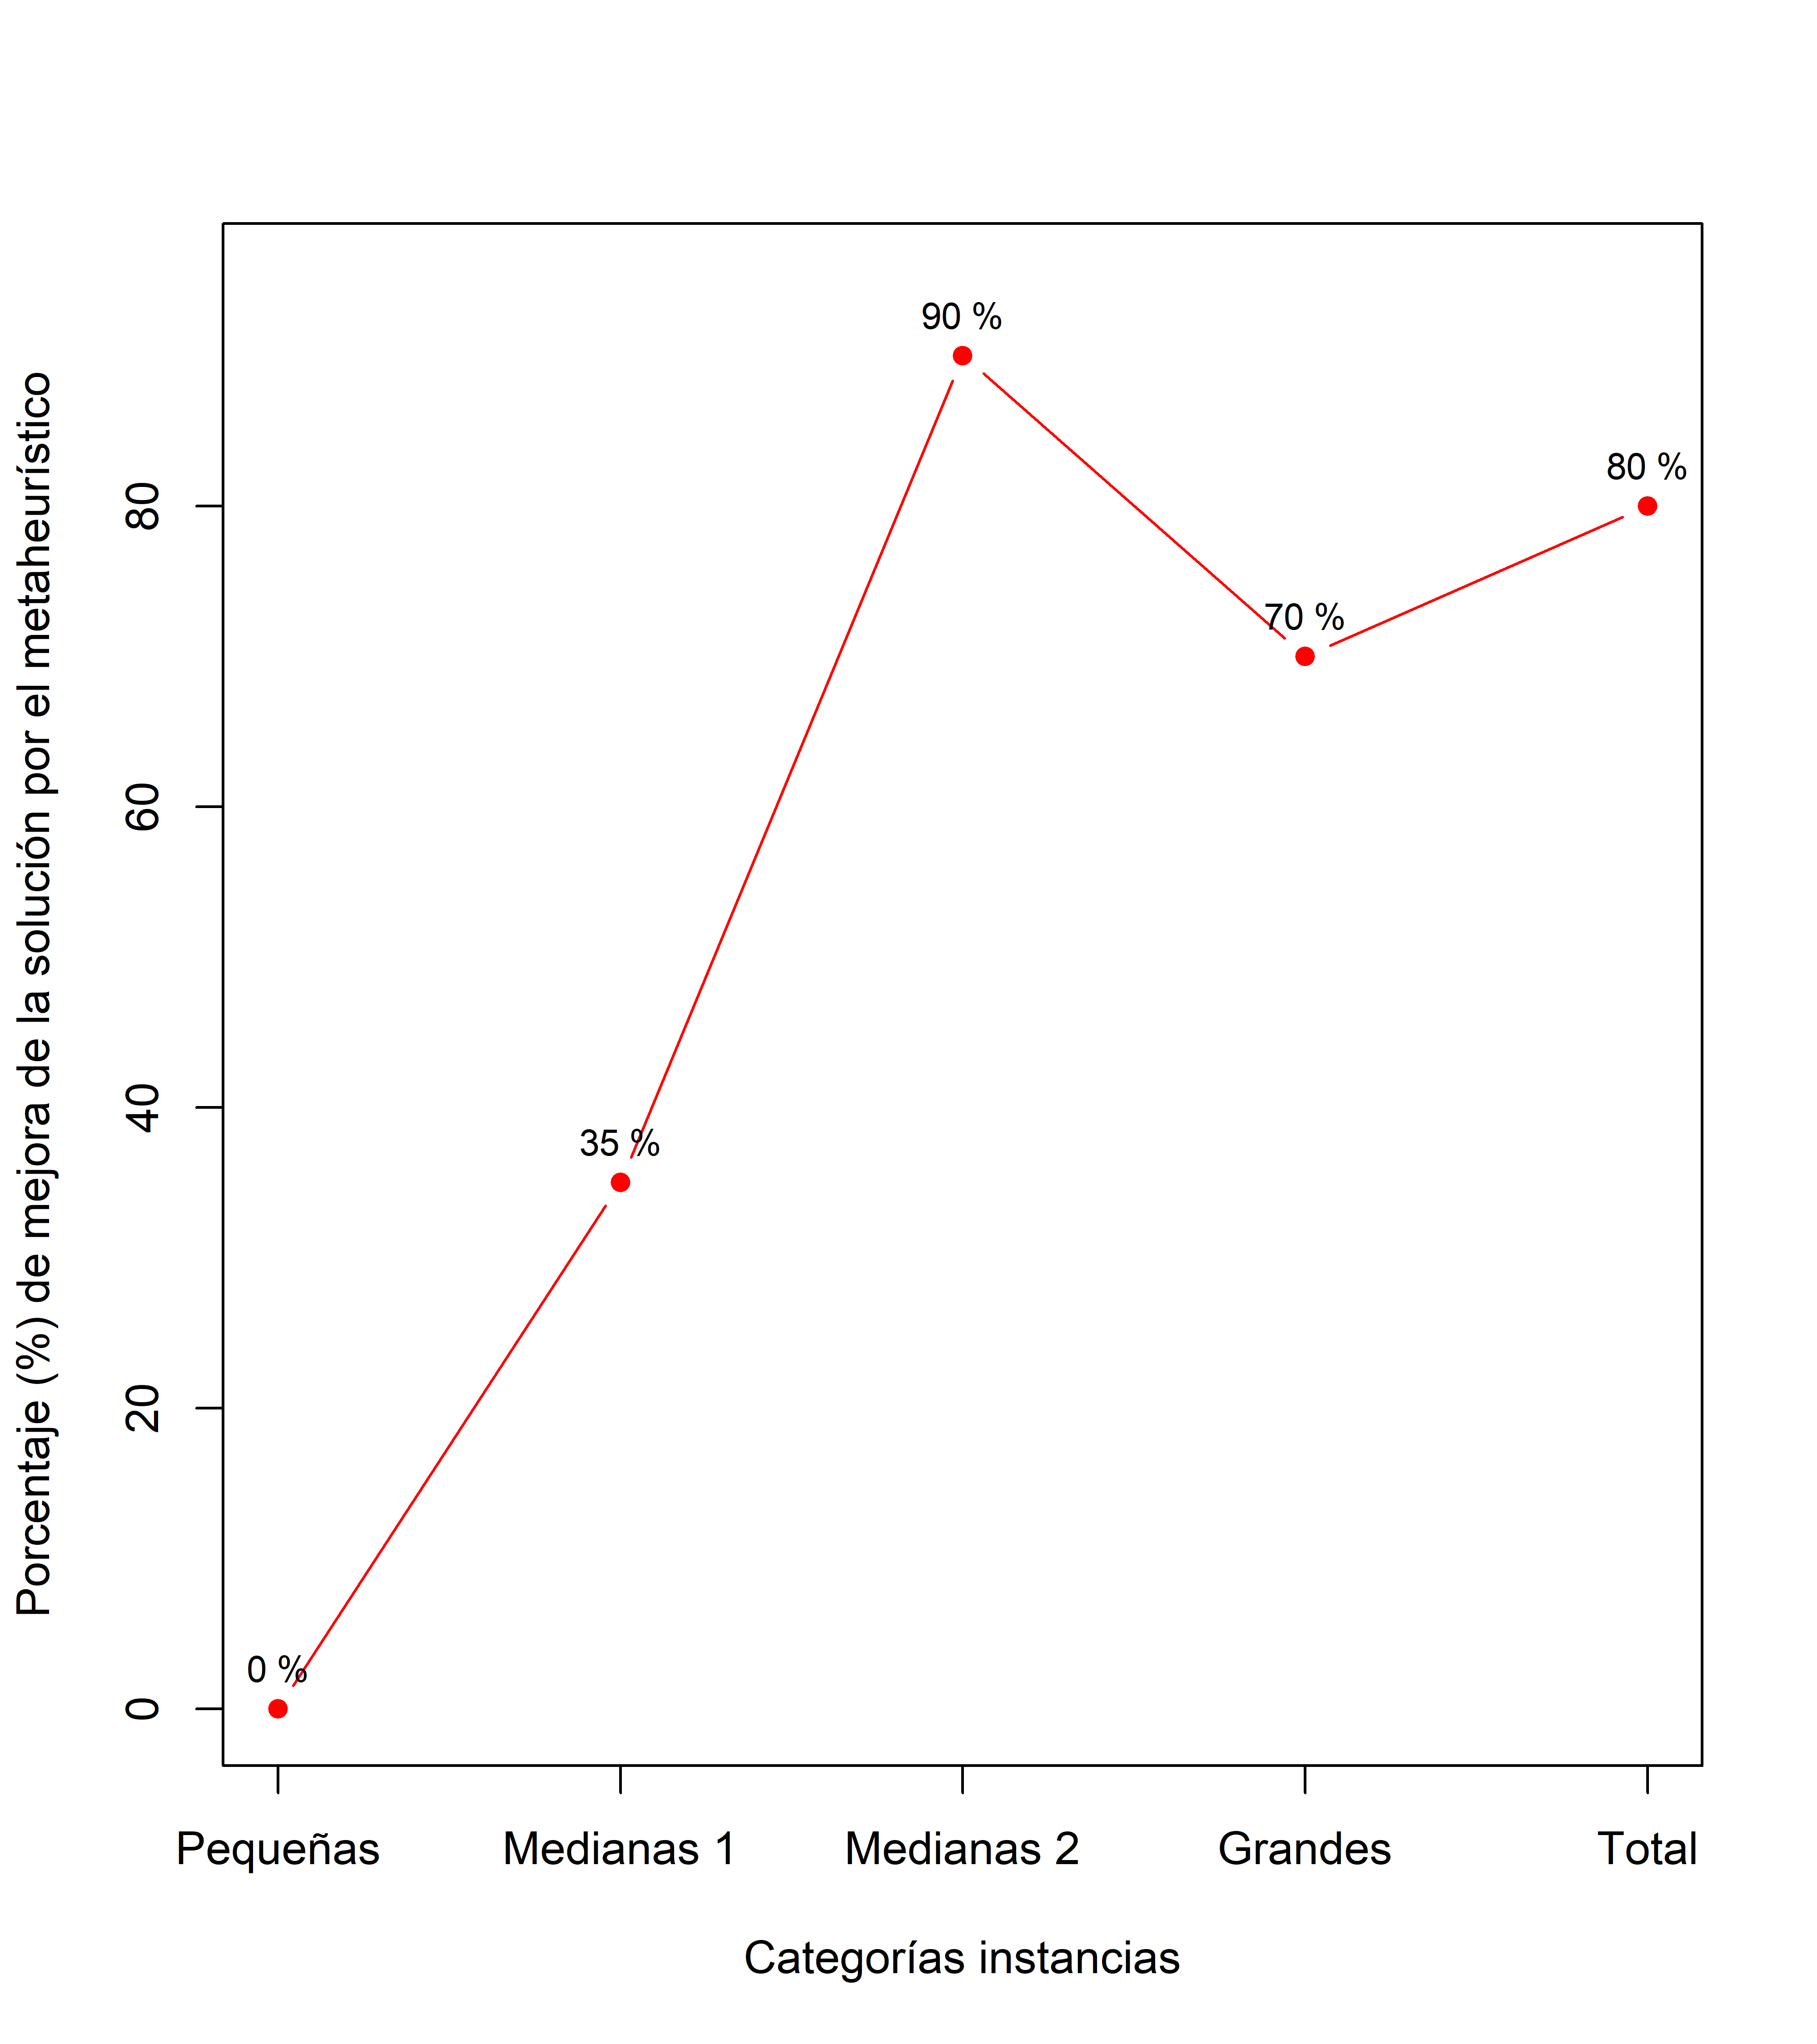
\includegraphics[scale = 0.6]{Figures/mejoras.png}
\caption{Comportamiento del porcentaje de mejora de la solución encontrada por la metaheurística por categorías de instancias}
\label{resumenmejoras}
\end{figure}

Ahora, por medio de la prueba de hipótesis para proporciones se determinará estadísticamente la cantidad de instancias en las la metaheurística encuentra una mejor solución. Esta prueba se realizará para el total de las instancias en las que el modelo matemático reportó una solución y por la categoría mediana (tipo $1$ y $2$). Las pequeñas ni las grandes se consideran ya que par a las primeras la prueba $t$ mostró que no hay mejora y para las segundas la solución de todas las instancias fue mejoradas por la metaheurística.

\subsection{\textbf{Prueba de hipótesis para proporciones}}

La información del cuadro \ref{proporciones} se empleó para hacer la prueba de hipótesis para proporciones considerando un $\alpha = 0.05$, es decir, con un intervalo de confianza del $95\%$. Se espera que del total de los casos (por categoría y global) un mínimo del $60\%$ sean detectados como mejoras. Cabe mencionar que para los casos donde la metaheurística encontró la misma solución que el modelo, se tomará como mejora ya que el tiempo de ejecución de la metaheurística es considerablemente menor que el requerido por el modelo para encontrar una solución.


\begin{table}[htp]
\caption{Parámetros prueba de hipótesis para proporcioness}
\centering
\begin{tabular}{|l|c|c|c|}
\hline
\textbf{Categorías}        & \textbf{\begin{tabular}[c]{@{}c@{}}Número de \\ instancias\\ $n$\end{tabular}} & \textbf{\begin{tabular}[c]{@{}c@{}}Instancias observadas\\ con mejora\\ $x$\end{tabular}} & \textbf{\begin{tabular}[c]{@{}c@{}}Proporción de \\ instancias con mejora \\ $\hat{\theta} = x/n$\end{tabular}} \\ \hline
\textbf{Medianas tipo $1$} & 77                                                                             & 67                                                                                        & 0.870                                                                                                           \\ \hline
\textbf{Medianas tipo $2$} & 49                                                                             & 48                                                                                        & 0.980                                                                                                           \\ \hline
\textbf{Total instancias}  & 185                                                                            & 173                                                                                       & 0.935                                                                                                           \\ \hline
\end{tabular}
\label{resultados}
\end{table}

Se realizó el cálculo analítico con base en la ecuación \ref{pruebaprop} y como criterio de prueba para las proporciones la información del cuadro \ref{proporciones}. También se utilizó el programa R para aplicar esta prueba mediante la función \texttt{prop.test}. \\

\noindent \textbf{Instancias medianas tipo $1$} \\

Sea $H_{0}$: $\theta = \theta_{0}$ como hipótesis nula y como alternativa $H_{1}:\theta > \theta_{0}$, es decir, se demostrará estadísticamente que la metaheurística cumple con los cantidad de casos esperados, por lo tanto, los datos necesarios para emplear el criterio son $n = 77$, $\theta_{0} = 0.6$ y $\hat{\theta} = 0.870$ (datos del cuadro \ref{resumen}. Reemplazando los datos anteriores en la ecuación \ref{pruebaprop} se tiene que:
\begin{align}
\nonumber
    t & =  \frac{0.870 - 0.60}{\sqrt{(0.60(1-0.6))/77}} = 4.839. \\ \nonumber
\end{align}

Ahora, el valor de $z_{\alpha} = 1.645$ (valor más exacto de acuerdo a la tabla de distribución $z$ consultada en \citet{walpole}), por lo tanto, como $4.839 > 1.645$ rechazamos la $H_{0}$ lo que significa que la proporción de instancias mejoradas por la metaheurística en las instancias medianas tipo $1$ es de por lo menos un $60\%$. Aplicando la función \texttt{prop.test} en el programa R se puede observar que el valor $p < 0.05$.

\VerbatimInput{Resulpruebas/proporcionesmed1.txt}

El anterior procedimiento se repite para las categorías medianas tipo $2$ y para el total de las instancias, los resultados se consolidan en el cuadro \ref{resultadospropo}.

\begin{table}[htp]
\caption{Resultados prueba de hipótesis para las proporciones}
\centering
\begin{tabular}{|l|c|c|c|}
\hline
\textbf{Categorías}        & \textbf{Prueba   de hipótesis}                                                                                         & \textbf{\begin{tabular}[c]{@{}c@{}}Criterio de rechazo \\ $z > z_{alpha}$\end{tabular}} & \textbf{\begin{tabular}[c]{@{}c@{}}Rechazo de \\ la $H_{0}$\end{tabular}} \\ \hline
\textbf{Medianas tipo $2$} & \multirow{2}{*}{\begin{tabular}[c]{@{}c@{}}$H_{0}:   \theta = \theta_{0}$\\ $H_{1}: \theta > \theta_{0}$\end{tabular}} & $ 5.424 > 1.645$                                                                        & Si                                                                        \\ \cline{1-1} \cline{3-4} 
\textbf{Total instancias}  &                                                                                                                        & $9.304 > 1.645$                                                                         & Si                                                                        \\ \hline
\end{tabular}
\label{resultadospropo}
\end{table}

De acuerdo al cuadro \ref{resultadospropo}, se puede determinar estadísticamente que tanto para la categoría medianas tipo $2$ como para el total de instancias, la proporción de instancias mejoradas por la metaheurística es de por lo menos un $60\%$. 

\section{Conclusiones} \label{conclusiones}

Las decisiones de la ubicación de almacenamiento de los productos, son de vital importancia para determinar su facilidad de acceso, por lo tanto, contar con una herramienta que permita obtener un correcto acomodo, con base en criterios como el peso de los productos, cumplimiento de demanda, entre otros, es uno de los factores principales que permite realizar la recolección de pedidos en tiempo y forma y con ello mantener un nivel de respuesta rápida a la solicitud de los clientes.

Con las pruebas de hipótesis de medias de diferencia y de proporciones se comprueba estadísticamente que la metaheurística propuesta para solucionar de manera simultánea la ubicación de almacenamiento y las rutas de recolección con base a la prioridad de peso de las cajas de los productos y cumplimiento de demanda presenta mejores resultados que las soluciones reportadas hasta el momento por el modelo matemático, principalmente en las instancias que presentaron una mayor complejidad computacional.

Como trabajo futuro ya que se comprobó estadísticamente que las metaheurística mejora las soluciones encontradas hasta el momento por el modelo, sería interesante que estas soluciones fueran soluciones iniciales del método exacto en las instancias de altos complejos para mejorar el tiempo computacional y encontrar soluciones óptimas al problema y mediante el uso de las pruebas de hipótesis comprobar si la combinación de estos métodos aportan mejores soluciones que las encontradas hasta el momento para este tipo de problemas.

\section{Agradecimientos}
Al Consejo de Ciencia y Tecnología (CONACYT) y a la Universidad Autónoma de Nuevo León por apoyarme con la beca que me permite realizar mis estudios, a la Dra. Elisa Schaeffer por sus enseñanzas y conocimientos transmitidos durante la clase de modelos probabilísticos aplicados (semestre agosto 2020 - enero 2021) y a las Dra. María Angélica Salazar Aguilar y Dra. Jania Astrid Saucedo Martínez por su apoyo y asesoría durante este proyecto.

%% If you have bibdatabase file and want bibtex to generate the
%% bibitems, please use
%%
%\bibliographystyle{elsarticle-num-names} 
\bibliographystyle{achemso} 
\bibliography{refproyectoproba}

%% else use the following coding to input the bibitems directly in the
%% TeX file.

%\begin{thebibliography}{00}

%% \bibitem{label}
%% Text of bibliographic item

%\bibitem{}

%\end{thebibliography}
\end{document}
\endinput
%%
%% End of file `elsarticle-template-num.tex'.
